\documentclass{article}
\usepackage[utf8]{inputenc}
\usepackage[T1]{fontenc}
\usepackage{graphicx}
\usepackage{hyperref}
\usepackage{geometry}
\geometry{margin=1in}

\title{JILLIEFREE}
\date{Encyclopaedia Britannica (1771)}

\begin{document}
\maketitle

\section*{Historical source}
\textbf{Entry ID:} \texttt{entry-jilliefree-493} \\
\textbf{Volume ID:} 192984257 \\
\textbf{Character Count:} 1197

\subsection*{Extracted Text}
JILLIEFREE, a town on the northern bank of the river Cambia, opposite to James’s island, where the English had formerly a small part. The kingdom of Barrs, in which it is situated, produces abundance of the necessities of life; but the chief trade of the inhabitants in salt, which they carry up the river in mossy and, in recent bring them Italian corn, cotton-colby, elephants teeth, small quantities of gold duty. See. The number of causes and people continually employed in this trade, make the king of Barrs, according to Mr Park, more formalable or European, then one other definition on the river, and have encouraged him to establish those extravaguard duties, which traders of all nations are obliged to pay the entry, assuming almost 30:2), and wasn't great and small. These duties are commonly collected in person by the governor of Jillifires, who is attended by a troublesome train in diplomats, who have some knowledge of the English language, in consequence of their intercourse with them, and be well such importantly, that renders are often under the necessity of supplying with their demands, in order to get rid of them. N. Lat. 13: 16. W. Song. 16, 15, from Greenwich.

Jillice



\section*{Source record}
\begin{itemize}
\item \textbf{Dataset:} \texttt{NationalLibraryOfScotland/encyclopaedia\_britannica\_illustrated}
\item \textbf{Dataset Revision:} \texttt{309f765b1ecc83e0a7f7762e44b4a927a7555443}
\item \textbf{Page ID:} \texttt{britannica:309f765b1ecc83e0a7f7762e44b4a927a7555443:train:493} \\
  \textbf{Filename:} \texttt{page-0493-29246f4d055a.jpg} \\
  \textbf{Row Index:} 493 \\
  \textbf{SHA256:} \texttt{29246f4d055a2249...}
\end{itemize}

\begin{figure}[h]
\centering
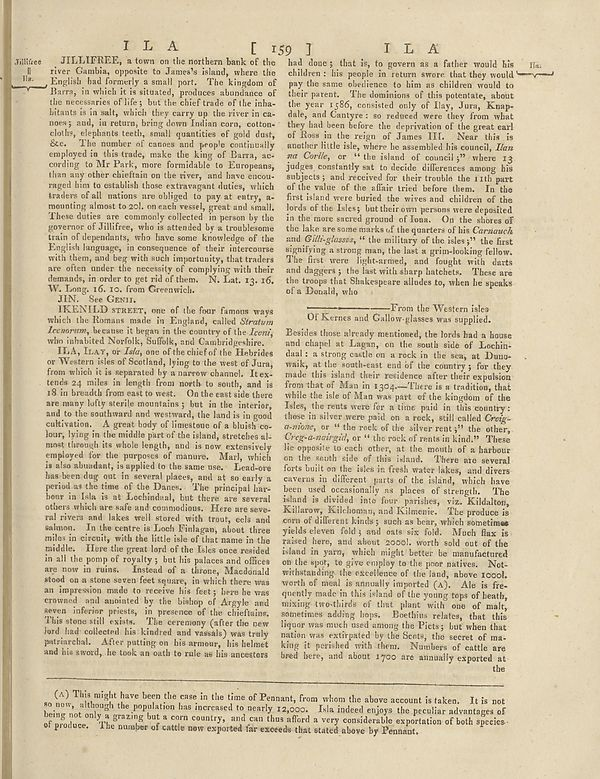
\includegraphics[width=0.85\textwidth]{../scans/page-0493-29246f4d055a.jpg}
\caption*{Source scan: \texttt{page-0493-29246f4d055a.jpg}}
\end{figure}

\end{document}
